\chapter{Marco Teórico}

Este capítulo va a poner en contexto al lector con respecto a conceptos básicos de criptografía para posteriormente explicar los algoritmos que van a ser implementados en el FPGA.\footnote{Según el ISO 7498-2 los términos correctos para encriptar y desencriptar son cifrar y descifrar respectivamente.}

\section{Conceptos Básicos}
Según la Real Academia Española \cite{bruce} la criptografía se define como 
\newline
\newline
\emph{Arte de escribir con clave secreta o de un modo enigmático.}
\newline
\newline
El mensaje que se desea transmitir es usualmente llamado \textit{texto plano} o simplemente \textit{mensaje}. Este mensaje pasa por un proceso donde se disfraza el texto plano en un \textit{texto cifrado}, el proceso es llamado \textit{cifrado}. El proceso inverso donde se toma un texto cifrado en un texto plano se denomina \textit{descifrado}. 

El texto plano o mensaje se denota usualmente por la letra M o P, el texto cifrado se denota usualmente por la letra C, la función o algoritmo que cifra se denota por E y la que descrifa se denota por D. Un algoritmo criptográfico corresponde a la función matemática para cifrar y descrifrar.
\newline
Se muestra en las Ecuaciones \eqref{eqCifrado} y \eqref{eqDescifrado} las relaciones entre estas notaciones. Note como al aplicarle la función de cifrado al texto plano se obtiene el texto cifrado y como al aplicarle la función de descifrado al texto cifrado se obtiene el texto plano. Finalmente se debe cumplir la identidad que describe la Ecuación \eqref{eqCifraDescifra}. \cite{bruce}
\begin{equation} \label{eqCifrado}
E(M) = C
\end{equation}
\begin{equation} \label{eqDescifrado}
D(C) = M
\end{equation}
\begin{equation} \label{eqCifraDescifra}
D(E(M)) = M
\end{equation}


La importancia de criptografía transciende más allá de brindar la confidencialidad en la comunicación la criptografía también cumple con la siguientes tareas:
\begin{itemize}
\item Autenticación: El receptor del mensaje debe de poder conocer y asegurar el emisor del mensaje, esto para que un tercero no pueda adjudicarse la identidad del emisor.
\item Integridad: El receptor tiene que poder asegurarse que el mensaje no fue cambiado en el transito del mismo. Esto para que un tercero no pueda cambiar el contenido enviado por el emisor sin que el receptor lo sepa.
\item \textit{Non-repudiation}: El emisor del mensaje no puede negar que el mensaje fue enviado por él. 
\end{itemize}

\section{Sistema criptográfico (\textit{criptosistema})}
Cuando la seguridad del algoritmo se basa en como procede el algoritmo, se denomina \textit{algoritmo restringido}. Este tipo de algoritmos son poco utilizados en la actualidad debido al gran problema que presentan. Tomemos de ejemplo que un grupo de usuarios decide utilizar un algoritmo de cifrado restringido para sus comunicaciones, se tendrá una comunicación segura hasta que alguno de los miembros decida salirse del grupo, ya que el usuario al no pertenecer más al grupo, no le importa mantener en secreto el algoritmo y puede distribuirlo para que terceros intercepen las comunicaciones. Así cada vez que un miembro deja el grupo, el grupo debe proceder a cambiarse a todo un nuevo algoritmo lo cual puede tornarse una labor complicada.

En cambio, la criptografía moderna \cite{denning} agrega el concepto de \textit{llave} donde se tiene un algoritmo el cual toma como parámetro de entrada una llave y el texto plano o texto cifrado y cifra o descifra el mismo de forma correcta únicamente si se tiene la llave correcta. Retomando el ejemplo anterior, el grupo solamente necesitaría cambiar de llave cuando un miembro se va, facilitando el uso del cifrado y manteniendo las comunicaciones secretas.

Este concepto anterior viene a definir lo que actualmente se conoce como sistema criptográfico o \textit{criptosistema}. Según \cite{denning} un criptosistema cuenta con 5 componentes:
\begin{itemize}
\item Un espacio de textos planos o mensajes ($M$)
\item Un espacio de textos cifrados ($C$)
\item Un espacio de llaves ($k$)
\item Una familia de \textit{transformaciones de cifrado}: $E_K: M\rightarrow C$ donde $K \epsilon  k$
\item Una familia de \textit{transformaciones de descrifrado}: $C_K: C\rightarrow M$ donde $K \epsilon  k$
\end{itemize} 


Se entiende como \textit{espacio} el conjunto de posibles valores para la variable dada, sea esta M, C o K.
Y una familia de transformaciones corresponde a todos los posibles mapeos que se pueden realizar de un espacio a otro (de $M$ a $C$ o viceversa) con todos los valores contenidos en el espacio $k$.

\begin{figure}
	\centering
	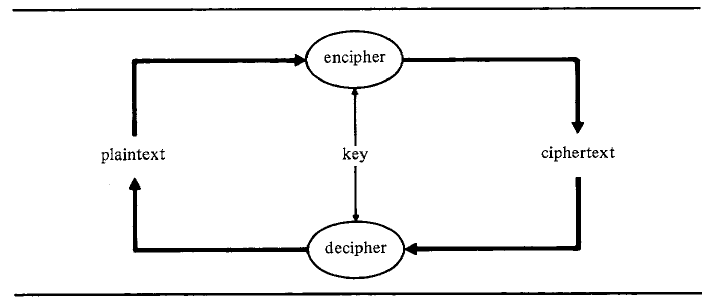
\includegraphics[width=0.8\textwidth]{./images/figExplicacionSistemaCripto}
	\caption{Descripción gráfica de un sistema criptográfico.}
	\label{figExplicacionSistemaCripto}
\end{figure}


En la actualidad se trabaja la criptografía sobre computadoras, es decir, cifrando y descrifrando bits, los cuales pueden tener diferentes significados, ya sea una imagen, un texto, un programa, etc. Esto significa que en la actualidad no se trabaja sobre caracteres del alfabeto o símbolos, sino más bien sobre 1's y 0's. Esto toma relevancia ya que al tener solo dos símbolos para cifrar, los algoritmos se vuelven más complejos por la falta de alternativas para sustituir un símbolo por otro.

Así antiguamente la criptografía se basaba en caracteres que eran sustituidos o traspuestos por otros caracteres. Esto corresponde a cifrados de sustitución y de transposición, los cuales continúan siendo la base de la criptografía pero basado los 2 símbolos del sistema binario.

Como se explicó anteriormente este tipo de cifrado se basa en tomar un caracter del texto plano y sustituirlo por otro caracter. Para descrifrar el texto cifrado simplemente se sustituyen de vuelta los caracteres y listo.

Según \cite{bruce} en la criptografía clásica existen 4 tipos de cifrado por sustitución:
\begin{itemize}
\item Cifrado de sustitución simple: Una sustitución de uno a uno entre cada caracter del texto plano y el texto cifrado.
Ejemplos de este tipo de sustitución son el famoso cifrado de César y el ROT13 utilizado en UNIX.

\item Cifrado de sustitución homofónico: Una sustición de uno a muchos. Un caracter del texto plano, por ejemplo A, puede ser sustituido por varios caracteres en el texto crifado, por ejemplo ``5'', ``13'', ``43''. Observe la Figura \ref{figExampleHomophonicCipher} donde se presenta una serie de posibles asignaciones de números a las letras del mensaje PLAIN PILOT y un posible texto cifrado haciendo uso de este tipo de cifrado.

\begin{figure}
	\centering
	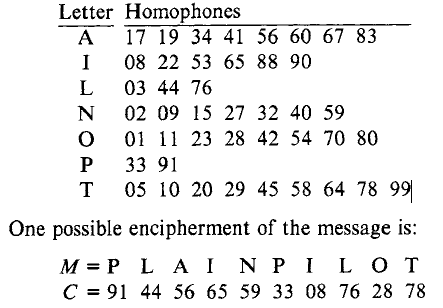
\includegraphics[width=0.6\textwidth]{./images/figExampleHomophonicCipher}
	\caption{Ejemplo de cifrado homofónico.}
	\label{figExampleHomophonicCipher}
\end{figure}


\item Cifrado de sustitución de poligrama: Una sustitución por bloques en donde se toma un bloque de caracteres del texto plano y se sustituye por su bloque equivalente en el texto cifrado. Por ejemplo si en el texto plano se tiene ``ABC'' se sustituye por ``SLL'' en el texto cifrado.

\item Cifrado de sustitución polialfabético: ????? 
\end{itemize}

La otra variedad de algoritmos son los de tranposición, en este tipo de algoritmos de cifrado el texto plano se convierte en texto cifrado cuando el orden de los caracteres es cambiado bajo alguna norma. Un ejemplo moderno de este tipo de algoritmos es el ``rail-fence" donde el texto plano se reacomoda con la forma de una cerca como se observa en la Figura \ref{figExampleTranspositionCipher}. En este caso la llave del algoritmos sería la profundidad de la cerca, para efectos de este ejemplo es de 3.

\begin{figure}
	\centering
	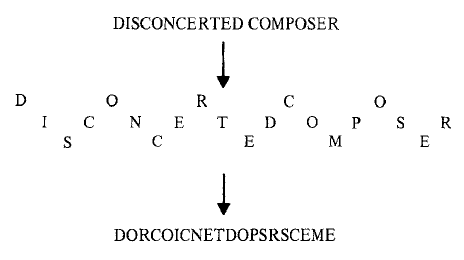
\includegraphics[width=0.65\textwidth]{./images/figExampleTranspositionCipher}
	\caption{Ejemplo de cifrado de transposición.}
	\label{figExampleTranspositionCipher}
\end{figure}


Actualmente en los algoritmos que se implementan en computadoras se combina tanto la tranposición como la sustitución. Por ejemplo se tiene el algoritmo RC5, el cual se desarrollará más adelante en este proyecto en donde se utiliza corrimientos o rotaciones a bits (tranposición) y sumas o XOR's (sustituciones) para cifrar el texto plano. Los algoritmos que se implementan en la criptografía se dividen en 2 categorías principales: simétricos y de llave pública (también llamados asimétricos \cite{???}).


\section{Algoritmos de cifrado}
\subsection{Algoritmos simétricos}
\cite{bruce} da una muy buena analogía para explicar el concepto de un algoritmo simétrico. Piense en el algoritmo como una caja fuerte. La combinación de la caja fuerte vendría a ser la \textit{llave} del algoritmo. Note como en una caja fuerte cualquier persona con la combinación puede llegar, abrir la caja y poner o sacar documentos de la misma. En el caso de no conocer la combinación, se debe proceder a forzar la caja o probando todas las combinaciones posibles hasta hallar la correcta. Es decir en un algoritmo simétrico se cuenta con una llave única que funciona tanto para cifrar como para descrifrar los mensajes como se muestra en la Figura \ref{figSimmetricKeyAlgorithm}. La notación para el cifrado y descrifado en estos algoritmos se muestra en las Ecuaciones \eqref{eqCifradoSimetrico} y \eqref{eqDescifradoSimetrico}.
\begin{equation}\label{eqCifradoSimetrico}
E_K (M) = C
\end{equation}

\begin{equation}\label{eqDescifradoSimetrico}
D_K (C) = M
\end{equation}


\begin{figure}
	\centering
	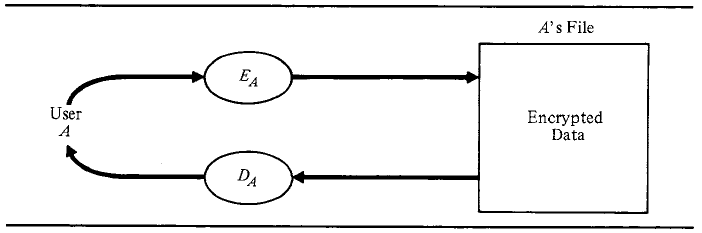
\includegraphics[width=0.9\textwidth]{./images/figSimmetricKeyAlgorithm}
	\caption{Descripción gráfica de una algoritmo de llave simétrica.}
	\label{figSimmetricKeyAlgorithm}
\end{figure}


Los algoritmos simétricos se dividen en 2 categorías (\cite{bruce}):

\begin{itemize}
\item Cifrado de bloque: Se cifra en bloques de bits ya sea bytes, words, etc. Es decir cuando se va a proceder a cifrar un texto plano, se segmenta el texto en grupos de bits y estos son cifrados de manera independiente. Se puede tomar como ejemplo el algoritmo \textit{Data Encryption Standart} (DES) el cual cifra sobre bloques de 64 bits. Ejemplos de estos algoritmos pueden ser:
\begin{itemize}
\item Data Encryption Standart (DES).
\item Lucifer.
\item LOKI.
\item 3-way.
\item RC5.
\item GOST.
\item IDEA.
\end{itemize}

\item Cifrado de \textit{Stream}: Es cuando se trabaja sobre un bit únicamente. Estos no son muy usuales en la actualidad ya que al trabajar en lenguaje binario solo se cuenta con 2 símbolos y si se cifra únicamente un bit no existen muchas posibilidades para sustituir o transposicionar.
Ejemplos de estos algoritmos pueden ser:
\begin{itemize}
\item RC4.
\item SEAL.
\item WAKE.
\end{itemize}
\end{itemize}

Según (\cite{bruce}) los criptosistemas simétricos en la red afrontan los siguientes problemas
\begin{itemize}
\item Distribución de la llave: La llave se debe mantener en secreto. Esto en la actualidad en una tarea demasiado díficil de lograr porque la llave debe ser conocida para el cifrado y descifrado (emisores y receptores) entonces para establecer una comunicación segura el primer paso debe ser entregar la llave de forma segura, lo cual en una red de computadoras se puede tornar una tarea prácticamente imposible de realizar. La única solución sería entregar las llaves mediantes un servicio de \textit{courier} o similares e igualmente se corren riesgos. 

\item Compromiso de seguridad: Si la llave es conocida por un tercero, si este intercepta el tráfico de información, todas las comunicaciones serán descifradas fácilmente.

\item Comunicaciones aisladas: En el caso de que cada usuario de una red se desee comunicar secretamente por separado con todos los otros usuarios del misma haciendo uso del mismo criptosistema, se debe utilizar una llave diferente para cada comunicación. Así para una red de N usuarios se requieren $N(N - 1)/2$ llaves. A primera vista esto no parece tan importante pero por ejemplo para 10 usuarios, se necesitan 45 llaves lo cual está bien, pero para 100 usuarios se necesitarían 4950 llaves.
\end{itemize}



\subsection{Algoritmos de llave pública}
Nuevamente \cite{bruce} nos ofrece una excelente analogía para explicar en este caso los algoritmos de llave pública. Tenemos un \textit{mailbox}, donde cualquier persona puede poner un mensaje adentro pero ÚNICAMENTE el dueño puede abrirlo para sacar y leer los mensajes.
\newline
\newline
En los algoritmos de llave pública los emisores hacen uso de una llave para cifrar los mensajes que desean enviar pero estos mensajes pueden ser descrifrados únicamente si se tiene la llave para descifrar mensajes que es diferente de la llave para cifrar, la cual la tendrá el receptor bien resguardada. En la Figura \ref{figPublicKeyAlgorithm} se muestra el diagrama básico de un algoritmo de llave pública. Ejemplos de estos algoritmos pueden ser:
\begin{itemize}
\item RSA
\item Pohlig-Hellman
\item Rabin
\item ElGamal
\end{itemize}

\begin{figure}
	\centering
	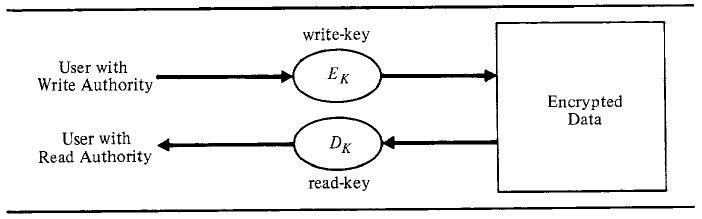
\includegraphics[width=0.65\textwidth]{./images/figPublicKeyAlgorithm}
	\caption{Descripción gráfica de una algoritmo de llave pública.}
	\label{figPublicKeyAlgorithm}
\end{figure}

Estos algoritmos sientan su base matemática en funciones llamadas \textit{one-way} en donde al aplicarle una función a una variable, la variable no puede retornar a su valor original de ninguna manera, es decir la función no tiene una inversa. 

Según \cite{bruce} existen funciones \textit{one-way} con una ``puerta trasera'' donde se puede retornar a la variable original, este tipo de funciones son las que se implementan en algoritmos de llave pública. para lograr este objetivo los algoritmos dominantes de esta rama se basan en la dificultad de factorizar números grandes que son el resultado de multiplicar dos números primos grandes como también se basan en el \textit{Discrete Logarithm Problem}.

En estos algoritmos no es posible a partir de la llave para cifrar obtener la llave para descrifrar. Esto permite que la llave para cifrar se pueda hacer pública, por lo cual recibe el nombre de llave pública y la llave para descrifrar se denomina llave privada. La notación para estos algoritmos corresponde a la de las Ecuaciones \eqref{eqCifradoPublico} y \eqref{eqDescfiradoPublico}
\begin{equation} \label{eqCifradoPublico}
E_{K_x} (M) = C
\end{equation}
\begin{equation} \label{eqDescfiradoPublico}
D_{K_y} (C) = M
\end{equation}

El objetivo de utilizar cifrado de llave pública se basa en:
\begin{itemize}
\item Receptor y emisor acuerdan un sistema de cifrado.
\item El receptor entrega al emisor su llave pública.
\item El emisor cifra el texto plano haciendo uso de la llave pública entregada y el sistema acordado.
\item El emisor envía el texto cifrado.
\item El receptor descrifa el texto cifrado haciendo uso de la llave privada.
\end{itemize}

De esta manera no hay forma que fisgones logren descrifrar el mensaje aunque obtengan la llave pública, así el receptor se asegura que las comunicaciones van a ser mucho más seguras ya que el emisor deja de tener la llave para descifrar y no puede brindarse a nadie o que sea robada a este. Para la implementación de un criptsistema que hace uso de algoritmo de llave pública, lo que se hace es que en la red se tiene una base de datos donde se registra el usuario y su respectiva llave pública, así cuando un usuario se desea comunicar con otro, va a la base de datos, busca al usuario y su llave pública, cifra el mensaje con la misma y se la envía. Esto solventa los problemas que presentaba anteriormente los algoritmos simétricos, ya que no es necesario transmitir de forma secreta llaves para poder realizar comunicaciones y para que diferentes usuarios se comuniquen de forma secreta entre si no es necesario el uso de diferentes llaves por cada enlace de comunicación. 

Algunos usos de estos algoritmos en la actualidad son:
\begin{itemize}
\item LLave maestra para el sistema de pago digital de un banco.
\item La clave que utiliza un gobierno para certificar sus visas o pasaportes.
\item La firma digital es un notario público.
\end{itemize} 

\subsection{Criptosistemas híbridos}
Los beneficios que conlleva utilizar algoritmos de llave pública son grandes pero se pagan a un precio muy alto: tiempo de procesamiento. Según \cite{bruce} el tiempo de procesamiento del RSA con respecto al del DES es de alrededor de 1000 mil veces más lento. 

En un mundo donde la velocidad es una clave fundamental en las comunicaciones se propuso la siguiente solución. Ya que los algoritmos simétricos tienen la debilidad de comunicar la llave antes de comenzar la comunicación pero son mucho más rápidos, y que los algoritmos de llave pública ostentan una mejor sistema para comunicarse en la red secretamente pero son muy lentos, se decidió utilizar ambos. La llave del algoritmo simétrico es encriptada con una algoritmo de llave pública para transmistirse en la red sin comprometerla y posterior a esto se realizan las comunicaciones con el algoritmo simétrico para obtener una mejor velocidad de comunicación. Se puede ver el protocolo de la siguiente manera (\cite{bruce}):
\begin{itemize}
\item El receptor envía su llave pública al emisor.
\item El emisor genera una llave de sesión\footnote{A common cryptographic technique is to encrypt each individual conversation with a separate key. This is called a session key, because it is used for only one
particular communications session. As discussed in Section 8.5, session keys
are useful because they only exist for the duration of the communication. How
this common session key gets into the hands of the conversants can be a
complicated matter.} la cifra y se la envía al receptor usando la llave pública que le fue dada.
\item El receptor descrifra la llave de sesión usando su llave privada.
\item Ahora ambos puede comunicarse de forma secreta con la llave de sesión con un criptosistema simétrico.
\end{itemize}





\section{Seguridad en algoritmos de cifrado}
Como parte de la investigación previa para este proyecto no podemos dejar de lado la otra cara de la moneda, el criptoanálisis. Claramente el objetivo de la criptografía es mantener un mensaje en secreto de terceros, pues el criptoanálisis según (\cite{raeAnalisis}) es el ``arte de descifrar criptogramas''. Así es como los terceros buscan inmiscuirse en las comunicaciones secretas sin tener un acceso a la llave, la ciencia que abarca la criptografía y el criptoanálisis es conocida como criptología (\cite{denning}). 

Según \cite{bruce}, el criptógrafo al diseñar su algoritmo debe asumir que el criptoanalista puede tener un acceso completo a las comunicaciones entre emisor y receptor y al algoritmo que implementa el criptosistema

Eavesdroppers are assumed to have complete access to the communications between the sender and receiver.

Cryptanalysis is the science of recovering the plaintext of a message without access to the key. Successful cryptanalysis may recover the plaintext or the key. It also may find weaknesses in a cryptosystem that eventually lead to the previous results. (The loss of a key through noncryptanalytic means is called a compromise.) An attempted cryptanalysis is called an attack. A fundamental assumption in cryptanalysis, first enunciated by the Dutchman A. Kerckhoffs in the nineteenth century, is that the secrecy must reside entirely in the key [794]. Kerckhoffs assumes that the cryptanalyst has complete details of the cryptographic algorithm and implementation. (Of course, one would assume that the CIA does not make a habit of telling Mossad about its cryptographic algorithms, but Mossad probably finds out anyway.) While real-world cryptanalysts don’t always have such detailed information, it’s a good assumption to make. If others can’t break an algorithm, even with knowledge of how it works, then they certainly won’t be able to break it without that knowledge. There are four general types of cryptanalytic attacks. Of course, each of them assumes that the cryptanalyst has complete knowledge of the encryption algorithm used:

\subsection{Tipos de ataques}

- Ciphertext-only attack.

- Known-plaintext attack
 
- Chosen-plaintext attack
 
- Adaptive-chosen-plaintext attack
 
- Chosen-ciphertext attack
 
- Chosen-key attack.
 
- Rubber-hose cryptanalysis



Public-key cryptosystems are vulnerable to chosen-plaintext attacks. If C = E(P), when P is one plaintext out of a set of n possible plaintexts, then a cryptanalyst only has to encrypt all n possible plaintexts and
compare the results with C (remember, the encryption key is public). He won’t be able to recover the decryption key this way, but he will be able to determine P.


\subsection{Tamaño de la llave}
Como se mencionó anteriormente la seguridad de un buen algoritmo depende del tamaño de su llave. 

Asumiendo que se tiene una seguridad del algoritmo perfecta, la única forma de quebrar el criptosistema sería mediante un ataque de fuerza bruta el cual es un tipo de ataque \textit{known-plaintext} donde sería solamente necesario unos 64 bits de texto plano y texto cifrado para ejecutarlo. Ahora tomemos en consideración el tamaño de la llave, si se tuviera una llave de $2^8$ bits el atacante solamente tendría que probar 256 posibilidades para obtener la llave lo que le tomaría a un atacante unos cuantos segundos en una computadora, en cambio para $2^{64}$ bits tenemos $1.8446744^{19}$ posibles llaves que el atacante debe probar lo cual tomaría con los recursos computacionales de una supercomputadora alrededor de 585,000 años. Y para una longitud de llave de 2048, con un billón de intentos por segundo en computadoras en paralelo se necesitarían  10597 años para encontrar la llave.

Comparar el nivel de seguridad antes un ataque de fuerza bruta de un algoritmo simétrico y uno de llave pública con llaves del mismo tamaño no es posible. La Figura \ref{figVariacionLlaves} muestra una tabla con equivalentes realizados empíricamente por \cite{bruce} sobre tamaños de llaves que dan un nivel de seguridad equivalente para los 2 tipso de algoritmos basado en los algoritmos más populares de cada rama.

\begin{figure}
	\centering
	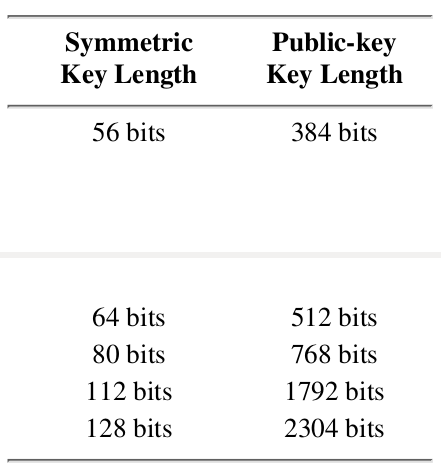
\includegraphics[width=0.65\textwidth]{./images/figVariacionLlaves}
	\caption{Comparación del tamaño de llaves en algoritmos simétricos y asimétricos.}
	\label{figVariacionLlaves}
\end{figure}

\subsection{Manejo de las llaves}
Se puede tener un algoritmo extremadamente robusto, veloz y con un tamaño de llave perfecto, pero si un atacante puede obtener la llave, ya sea chantajeando, interceptando, extorsionando o pagando por la misma se pierde todo. De ahí la gran importancia de como manejar las llaves.

Al ser esto tan importante existen ciertas maneras de generar llaves:
\begin{itemize}
\item Ingresada por el usuario: El usuario elige una llave y esa es la que se va a utilizar. Este método es sumamente inseguro
debido a que gran cantidad de contraseñas se repiten, o son datos personales del usuario como su número de celular o similares.
Por tanto se pueden realizar \textit{ataques de diccionario} donde las primeras llaves que se prueban son las mencionadas
anteriormente.

\item Random keys: Es un muy buen método para generar llaves, consiste en utilizar un programa que genere la llave, es ventajoso
ya que es robusto ante ataques de diccionario pero presenta el problema que la llave es difícil de recordar y posiblemente se olvide.

\item pass phrases: Es una combinación de ambos, el usuario escribe una contraseña fácil de recordar y después
hace uso de un one-way has function para convertir esta llave en una llave random de tamaño arbitrario.
\end{itemize}





\section{Escogencia de los algoritmos a implementar}
En un principio el objetivo de este proyecto era realizar una comparación con las métricas descritas en la Introducción sobre un algoritmo simétrico y un algoritmo de llave pública, posterior a la realización del marco teórico se llegó a la conclusión de que realizar este análisis no iba a ser para nada justo debido mayoritariamente a tres razones:
\begin{itemize}
\item El tiempo de procesamiento: Como se menciona anteriormente los algoritmos de llave pública consumen mucho más tiempo realizando el cifrado y descifrado que un algoritmo de llave simétrica.
\item La formas en las que estos algoritmos son diseñados producen falencias en seguridad distintas por lo cual analizar comparativamente no sería tan interesante.
\item Los algoritmos realizan el proceso de cifrado de maneras muy diferentes: En el caso de los algoritmos simétricos son basados en transposición y sustitución que trabajan en su mayoría con XOR's, sumas y corrimientos. En cambio los algoritmos de llave pública trabajan  basados en la multiplicación de números primos y \textit{Discrete Logarithm Problem} donde ocurren muchas multiplicaciones y sumas. Esto produce un consumo de recursos muy diferente entre ambos tipos.
\end{itemize}

Bajo el criterio que ambos algoritmos tuvieran características similares para poder ser analizados comparativamente y que fueran fáciles de implementar a nivel de hardware se optó por comparar dos algoritmos simétricos, específicamente el RC5 y el IDEA los cuales están basados en redes de Feistel\footnote{Feistel Networks
Most block algorithms are Feistel networks. This idea dates from the early
1970s [552,553]. Take a block of length n and divide it into two halves of
length n/2: L and R. Of course, n must be even. You can define an iterated
block cipher where the output of the ith round is determined from the output of
the previous round:
Li = Ri - 1
Ri = Li - 1  f(Ri - 1,Ki)
Ki is the subkey used in the ith round and f is an arbitrary round function.
You’ve seen this concept in DES, Lucifer, FEAL, Khufu, Khafre, LOKI,
GOST, CAST, Blowfish, and others. Why is it such a big deal? The function is
guaranteed to be reversible. Because XOR is used to combine the left half with
the output of the round function, it is necessarily true that
Li - 1  f(Ri - 1,Ki)  f(Ri - 1,Ki) = Li - 1
A cipher that uses this construction is guaranteed to be invertible as long as the
inputs to f in each round can be reconstructed. It doesn’t matter what f is; f
need not be invertible. We can design f to be as complicated as we please, and
we don’t have to implement two different algorithms—one for encryption and
another for decryption. The structure of a Feistel network takes care of all this
automatically.
} y por tanto comparten características de diseño para que la comparación sea un poco más justa.



\section{Descripción de los algoritmos a implementar}
\subsection{RC5}


\subsection{IDEA o LUCIFER o FEAL}






\section{Características de un FPGA}



